\documentclass[10pt]{beamer}\usepackage[]{graphicx}\usepackage[]{color}
% maxwidth is the original width if it is less than linewidth
% otherwise use linewidth (to make sure the graphics do not exceed the margin)
\makeatletter
\def\maxwidth{ %
  \ifdim\Gin@nat@width>\linewidth
    \linewidth
  \else
    \Gin@nat@width
  \fi
}
\makeatother

\definecolor{fgcolor}{rgb}{0.345, 0.345, 0.345}
\newcommand{\hlnum}[1]{\textcolor[rgb]{0.686,0.059,0.569}{#1}}%
\newcommand{\hlstr}[1]{\textcolor[rgb]{0.192,0.494,0.8}{#1}}%
\newcommand{\hlcom}[1]{\textcolor[rgb]{0.678,0.584,0.686}{\textit{#1}}}%
\newcommand{\hlopt}[1]{\textcolor[rgb]{0,0,0}{#1}}%
\newcommand{\hlstd}[1]{\textcolor[rgb]{0.345,0.345,0.345}{#1}}%
\newcommand{\hlkwa}[1]{\textcolor[rgb]{0.161,0.373,0.58}{\textbf{#1}}}%
\newcommand{\hlkwb}[1]{\textcolor[rgb]{0.69,0.353,0.396}{#1}}%
\newcommand{\hlkwc}[1]{\textcolor[rgb]{0.333,0.667,0.333}{#1}}%
\newcommand{\hlkwd}[1]{\textcolor[rgb]{0.737,0.353,0.396}{\textbf{#1}}}%
\let\hlipl\hlkwb

\usepackage{framed}
\makeatletter
\newenvironment{kframe}{%
 \def\at@end@of@kframe{}%
 \ifinner\ifhmode%
  \def\at@end@of@kframe{\end{minipage}}%
  \begin{minipage}{\columnwidth}%
 \fi\fi%
 \def\FrameCommand##1{\hskip\@totalleftmargin \hskip-\fboxsep
 \colorbox{shadecolor}{##1}\hskip-\fboxsep
     % There is no \\@totalrightmargin, so:
     \hskip-\linewidth \hskip-\@totalleftmargin \hskip\columnwidth}%
 \MakeFramed {\advance\hsize-\width
   \@totalleftmargin\z@ \linewidth\hsize
   \@setminipage}}%
 {\par\unskip\endMakeFramed%
 \at@end@of@kframe}
\makeatother

\definecolor{shadecolor}{rgb}{.97, .97, .97}
\definecolor{messagecolor}{rgb}{0, 0, 0}
\definecolor{warningcolor}{rgb}{1, 0, 1}
\definecolor{errorcolor}{rgb}{1, 0, 0}
\newenvironment{knitrout}{}{} % an empty environment to be redefined in TeX

\usepackage{alltt}


%\input{slides_header.tex}
\usepackage{graphicx}
\usepackage{hyperref, url}
\hypersetup{colorlinks,citecolor=myorange,filecolor=red,linkcolor=brown,urlcolor=blue}

\usepackage{longtable,booktabs}
\usepackage{amssymb,amsmath}
\usepackage{animate}
\usepackage{subfig}
\usepackage{tikz}
\usetikzlibrary{shapes.geometric, arrows,shapes.symbols,decorations.pathreplacing}
\tikzstyle{startstop} = [rectangle, rounded corners, minimum width=3cm, minimum height=1cm, draw=black, fill=pinkish,text width=3.5cm]
\tikzstyle{startstop2} = [rectangle, rounded corners, minimum width=3cm, minimum height=1cm, draw=black, fill=background,text width=4.5cm]
\tikzstyle{startstop3} = [rectangle, rounded corners, minimum width=3cm, minimum height=1cm, draw=black, fill=beige,text width=3.0cm]
\tikzstyle{startstop4} = [rectangle, rounded corners, minimum width=3cm, minimum height=1cm, draw=black, fill=pinkish,text width=4.5cm]
\tikzstyle{io} = [trapezium, trapezium left angle=70, trapezium right angle=110, minimum width=2cm, minimum height=1cm, text centered, draw=black, fill=blue!30,text width=1.5cm]
\tikzstyle{process} = [rectangle, minimum width=1cm, minimum height=1cm, text centered, draw=black, fill=orange!30,text width=2cm]
\tikzstyle{decision} = [diamond, minimum width=2cm, minimum height=1cm, text centered, draw=black, fill=green!30]
\tikzstyle{arrow} = [thick,->,>=stealth]
\tikzstyle{both} = [thick,<->,>=stealth, red]


% used for tree of stats tests in 001-introduction
\tikzstyle{startstopstats} = [rectangle, rounded corners, minimum width=2cm, minimum height=.5cm,text centered, draw=black, fill=red!30]
\tikzstyle{iostats} = [trapezium, trapezium left angle=70, trapezium right angle=110, minimum width=2cm, minimum height=.5cm, text centered, draw=black, fill=blue!30]
\tikzstyle{processstats} = [rectangle, minimum width=1.5cm, minimum height=.5cm, text centered, draw=black, fill=orange!30]
\tikzstyle{processbigstats} = [rectangle, minimum width=1.5cm, minimum height=.5cm, text centered, draw=black, fill=orange!30,text width=1.6cm]
\tikzstyle{decisionstats} = [rectangle, minimum width=1cm, minimum height=1cm, text centered, draw=black, fill=green!30,text width=1.6cm]
\tikzstyle{decisionbigstats} = [rectangle, minimum width=1cm, minimum height=1cm, text centered, draw=black, fill=yellow!30,text width=2cm]

\usepackage{pifont}% http://ctan.org/pkg/pifont
\newcommand{\cmark}{\ding{51}}%
\newcommand{\xmark}{\ding{55}}%

\usepackage{ulem} % for strikeout

\usepackage{xcolor}
\usepackage{color, colortbl}
\definecolor{lightgray}{RGB}{200,200,200}
\definecolor{palegray}{RGB}{221,221,221}
\definecolor{myblue}{RGB}{0,89,179}
\definecolor{myorange}{rgb}{0.776,0.357,0.157}
\definecolor{gray}{RGB}{110,110,110}
\definecolor{darkgray}{RGB}{100,100,100}
\definecolor{lightgray}{RGB}{200,200,200}
\definecolor{palegray}{RGB}{221,221,221}
\definecolor{turquoise}{RGB}{81,193,188}
\definecolor{tomato}{RGB}{255,136,136}
\definecolor{mandarina}{RGB}{229,169,25}
\definecolor{foreground}{RGB}{81,141,193}
\definecolor{background}{RGB}{246,244,240}
\definecolor{highlight}{RGB}{229,169,25}
\definecolor{lowlight}{RGB}{200,200,200}
\definecolor{beige}{RGB}{255,255,240}
\definecolor{pinkish}{RGB}{255,223,247}
\definecolor{darktangerine}{rgb}{1.0, 0.66, 0.07}
\definecolor{deepink}{RGB}{255,20,147}
%\usepackage{shadethm}
%\colorlet{shadecolor}{blue!15}
%\colorlet{shadecolor}{palegray}
%\setlength{\shadeboxrule}{.4pt}

%\newshadetheorem{thm}{Theorem}
%\newshadetheorem{defm}{Definition}
%\newshadetheorem{exm}{Exercise}
%\newshadetheorem{remarkm}{Remark}
%\definecolor{shadethmcolor}{HTML}{EDF8FF}
%\definecolor{shadethmcolor}{RGB}{221,221,221}
%\definecolor{shaderulecolor}{HTML}{45CFFF}
%\definecolor{shaderulecolor}{RGB}{0,89,179}
%\setlength{\shadeboxrule}{.4pt}



\usepackage{epsfig}

\newcommand{\code}[1]{\texttt{#1}}
\newcommand{\blue}[1]{\textcolor{blue}{#1}}
\newcommand{\red}[1]{\textcolor{red}{#1}}

\usepackage{comment}

\makeatletter

\def \iqsssectiontitleheader {}

\newcommand{\iqsssectiontitle}[1]{
	\def \iqsssectiontitleheader{#1}
}

\@ifundefined{insertmainframenumber}
{%
	% \insertmainframenumber not defined
	\newcommand{\insertmainframenumber}{\inserttotalframenumber}
}
{%
	% \insertmainframenumber already defined
}%


\AtBeginSection[]{
	\title{\insertsectionhead}
	{
		%\definecolor{white}{RGB}{140,193,250}
		%\definecolor{white}{RGB}{200,200,200}
		%\definecolor{white}{RGB}{242,244,247}
		\definecolor{white}{RGB}{0,89,179}
		%\definecolor{iqss@orange}{rgb}{1,1,1}
		\ifnum \insertmainframenumber > \insertframenumber
		%\setbeamercolor{background canvas}{bg=myblue}
		%\setbeamercolor{normal text}{fg=black,bg=white}
		%\setbeamercolor{frametitle}{fg=red}
		%\setbeamercolor{section in toc}{fg=myblue, bg=white}
		%\setbeamercolor{subsection in toc}{fg=myblue, bg=white}
		\frame{
			\frametitle{\iqsssectiontitleheader}
			\tableofcontents[currentsection]
		}
		\else
		\frame{
			\frametitle{Backup Slides}
			\tableofcontents[sectionstyle=shaded/shaded,subsectionstyle=shaded/shaded/shaded]
		}
		\fi
	}
}
\makeatother
%\graphicspath{{/home/sahir/git_repositories/EPIB607/resources/assets/slides/figure/}}


\usepackage{fontspec}
%\setsansfont{Fira Sans}
%\setmonofont{Fira Mono}
%\setsansfont[ItalicFont={Fira Sans Light Italic},BoldFont={Fira Sans},BoldItalicFont={Fira Sans Italic}]{Fira Sans Light}
%\setmonofont[BoldFont={Fira Mono Medium}]{Fira Mono}

\def\installpath{/usr/local/share/texmf/fonts/opentype/libertinus/}
\setmainfont{LibertinusSerif}[
UprightFont    = *-Regular,
BoldFont       = *-Bold,
ItalicFont     = *-Italic,
BoldItalicFont = *-BoldItalic,
Ligatures      = TeX,
Extension      = .otf,
Path           = \installpath/
]

\setsansfont{LibertinusSerif}[
UprightFont    = *-Regular,
BoldFont       = *-Bold,
ItalicFont     = *-Italic,
BoldItalicFont = *-BoldItalic,
Ligatures      = TeX,
Extension      = .otf,
Path           = \installpath/
]


%\setmonofont{LibertinusSerif}[
%UprightFont    = *-Regular,
%BoldFont       = *-Bold,
%ItalicFont     = *-Italic,
%BoldItalicFont = *-BoldItalic,
%Ligatures      = TeX,
%Extension      = .otf,
%Path           = \installpath/
%]






\newcommand\Wider[2][3em]{%
	\makebox[\linewidth][c]{%
		\begin{minipage}{\dimexpr\textwidth+#1\relax}
			\raggedright#2
		\end{minipage}%
	}%
}


\newcommand {\framedgraphic}[1] {
	\begin{figure}
		\centering
		\includegraphics[width=\textwidth,height=0.9\textheight,keepaspectratio]{#1}
	\end{figure}
}


\newcommand {\framedgraphiccaption}[2] {
	\begin{figure}
		\centering
		\includegraphics[width=\textwidth,height=0.8\textheight,keepaspectratio]{#1}
		\caption{#2}
	\end{figure}
}




\setbeamercolor{itemize item}{fg=myblue}
\setbeamercolor{itemize subitem}{fg=myorange}
%\setbeamertemplate{itemize item}[square]
\setbeamertemplate{itemize item}[circle]
\setbeamertemplate{itemize subitem}[triangle]
\setbeamertemplate{blocks}[rounded][shadow=true]
\setbeamercolor{block body alerted}{bg=alerted text.fg!10}
\setbeamercolor{block title alerted}{bg=alerted text.fg!20}
\setbeamercolor{block body}{bg=structure!10}
\setbeamercolor{block title}{bg=structure!20}
\setbeamercolor{block body example}{bg=green!10}
\setbeamercolor{block title example}{bg=green!20}


\makeatletter
\newenvironment<>{proofs}[1][\proofname]{%
	\par
	\def\insertproofname{#1\@addpunct{.}}%
	\usebeamertemplate{proof begin}#2}
{\usebeamertemplate{proof end}}
\newenvironment<>{proofc}{%
	\setbeamertemplate{proof begin}{\begin{block}{}}
		\par
		\usebeamertemplate{proof begin}}
	{\usebeamertemplate{proof end}}
	\newenvironment<>{proofe}{%
		\par
		\pushQED{\qed}
		\setbeamertemplate{proof begin}{\begin{block}{}}
			\usebeamertemplate{proof begin}}
		{\popQED\usebeamertemplate{proof end}}
\makeatother


\makeatletter
\newenvironment<>{exams}[1][\proofname]{%
	\par
	\def\insertproofname{#1\@addpunct{.}}%
	\usebeamertemplate{example begin}#2}
{\usebeamertemplate{example end}}
\newenvironment<>{examc}{%
	\setbeamertemplate{exam begin}{\begin{block}{}}
		\par
		\usebeamertemplate{exam begin}}
	{\usebeamertemplate{exam end}}
	\newenvironment<>{exame}{%
		\par
		\pushQED{\qed}
		\setbeamertemplate{exam begin}{\begin{block}{}}
			\usebeamertemplate{exam begin}}
		{\popQED\usebeamertemplate{exam end}}
		\makeatother

%\definecolor{mycolor}{HTML}{F7F8E0}
%\declaretheorem[shaded={bgcolor=mandarina}]{theo}
%\declaretheorem[shaded={bgcolor=mycolor}]{propo}
%\declaretheorem[shaded={bgcolor=green!80!black!30}]{remark}

%\setbeamertemplate{navigation symbols}{\usebeamercolor[fg]{title in head/foot}\usebeamerfont{title in head/foot}\insertframenumber}


%\setbeamertemplate{footline}{}

\beamertemplatenavigationsymbolsempty % toggle off if you want navigation symbols at the bottom

\setbeamertemplate{footline}
{ \usebeamercolor[fg]{page number in head/foot}%
	\usebeamerfont{page number in head/foot}%
	\hspace{1em}\insertsectionhead%
	\hfill%
	\insertframenumber\,/\,\hyperlinkappendixstart{\insertmainframenumber}
	\ifnum \thepage = \insertframeendpage{\small .}\else{\phantom{\small .}}\fi
	\hspace{1em}
	\vskip2pt%
}

%\newtheorem{proposition}[theorem]{Proposition}
%\newtheorem{exercise}[theorem]{Exercise}
%\newtheorem{remark}[theorem]{Remark}


\usepackage{amsthm}
\usepackage{thmtools}

\setbeamertemplate{theorems}[ams style] 
%\setbeamertemplate{theorems}[numbered] 
%\setbeamertemplate{corollary}[numbered] 
\newtheorem{proposition}{Proposition}
\newtheorem{exercise}{Exercise}
\newtheorem{remark}{Remark}
\newtheorem{exam}{Example}
%\newtheorem{proof}{Proof}
%\newtheorem{corollaries}[theorem]{Corollary}
\newcommand*{\theorembreak}{\usebeamertemplate{theorem end}\framebreak\usebeamertemplate{theorem begin}}



\setlength{\emergencystretch}{3em} % prevent overfull lines
\providecommand{\tightlist}{%
	\setlength{\itemsep}{0pt}\setlength{\parskip}{0pt}}

\newcommand\AddButton{%
	\setbeamertemplate{background canvas}{%
		\begin{tikzpicture}[remember picture,overlay]
		\node[anchor=west] at ([yshift=5pt,xshift=0.1em]current page.south west)
		{\hyperlink{toc}{\beamergotobutton{back to TOC}}};
		\end{tikzpicture}%
	}%
}


\titlegraphic{\hfill
\includegraphics[height=1cm]{/home/sahir/git_repositories/EPIB607/slides/mcgill_logo.png}}




\graphicspath{{/home/sahir/git_repositories/epib607/inst/slides/figure/}}

%\let\oldShaded\Shaded
%\let\endoldShaded\endShaded
%\renewenvironment{Shaded}{\footnotesize\oldShaded}{\endoldShaded}

%\newcommand{\blue}[1]{\textcolor{blue}{#1}}
%\newcommand{\red}[1]{\textcolor{red}{#1}}


\usepackage{xparse}
\NewDocumentCommand\mylist{>{\SplitList{;}}m}
{
	\begin{itemize}
		\ProcessList{#1}{ \insertitem }
	\end{itemize}
}
\NewDocumentCommand\mynum{>{\SplitList{;}}m}
{
	\begin{enumerate}
		\ProcessList{#1}{ \insertitem }
	\end{enumerate}
}
\newcommand\insertitem[1]{\item #1}

\newcommand\FrameText[1]{%
	\begin{textblock*}{\paperwidth}(0pt,\textheight)
		\raggedright #1\hspace{.5em}
\end{textblock*}}
\IfFileExists{upquote.sty}{\usepackage{upquote}}{}
\begin{document}





\title{015 - Inference about a Population Mean ($\mu$)}
\author{EPIB 607}
\institute{
	Sahir Rai Bhatnagar\\
	Department of Epidemiology, Biostatistics, and Occupational Health\\
	McGill University\\
	
	\vspace{0.1 in}
	
	\texttt{sahir.bhatnagar@mcgill.ca}\\
	%\texttt{\url{https://sahirbhatnagar.com/EPIB607/}}
}

\date{slides compiled on \today}

\maketitle

%\section{Objectives}

\section{The t distribution}

\frame{\frametitle{Inference for $\mu$ when $\sigma$ is not known}
	Up until now, all of our calculations have relied on us knowing the
	value of the population standard deviation ($\sigma$). It is rare that this is the case. \\ \ \\
	
	We now consider methods of inference for when \blue{$\sigma$ is unknown}.
	\\ \ \\
	
	When $\sigma$ is unknown, we must \blue{estimate it from the data using $s$, the sample standard deviation}.
}

\frame{\frametitle{Inference for $\mu$ when $\sigma$ is unknown}
	\begin{itemize}
		\item When the true variance was known, we performed our calculations
		using the standardization \[Z =
		\frac{\overline{y}-\mu}{\sigma/\sqrt{n}} \sim \mathcal{N}(0,1).\] \pause 
		\item We no longer can use this, so instead we use \[t =
		\frac{\overline{y}-\mu}{s/\sqrt{n}} \sim t_{(n-1)}\] which follows a
		\textbf{$t$-distribution} with $n-1$ degrees of freedom based on the $n$ values, $y_1,...,y_n$ in an SRS \pause
		\item There is a different $t$ distribution for each sample size. The
		degrees of freedom specify which distribution we use, and are
		determined by the denominator used in estimating $s$ which is $(n-1)$.
\end{itemize} }


\begin{frame}{$\sigma$ known vs. unknown}
	\begin{center}
		\begin{tabular}{|l|c|c|} \hline
			$\sigma$& known & unknown \\ \hline Data & $\{y_1,y_2,...,y_n\}$ &
			$\{y_1,y_2,...,y_n\}$\\
			& & \\
			Pop'n param & $\mu$ & $\mu$\\
			& & \\
			Estimator & $\overline{y} = \frac{1}{n}\sum_{i=1}^n y_i$ & $\overline{y} = \frac{1}{n}\sum_{i=1}^n y_i$ \\
			& & \\
			SD & $\sigma$ & $s = \sqrt{\frac{\sum_{i=1}^n(y_i-\overline{y})^2}{n-1}}$ \\
			& & \\
			SEM & $\sigma/\sqrt{n}$ & $s / \sqrt{n}$ \\
			& & \\
			$(1-\alpha)100$\% CI & $\overline{y} \pm z^\star_{1-\alpha/2}$(SEM) & $\overline{y} \pm t^\star_{1-\alpha/2, (n-1)}$(SEM) \\
			& & \\
			test statistic & $\frac{\overline{y}-\mu_0}{\textrm{SEM}}\sim \mathcal{N}(0,1)$ &
			$\frac{\overline{y}-\mu_0}{\textrm{SEM}}\sim t_{(n-1)}$ \\
			\hline
		\end{tabular}
	\end{center}
\end{frame}



\begin{frame}{$t$ distribution vs. Normal distribution}
	
	\Wider[4em]{
		\begin{figure}
			\centering
			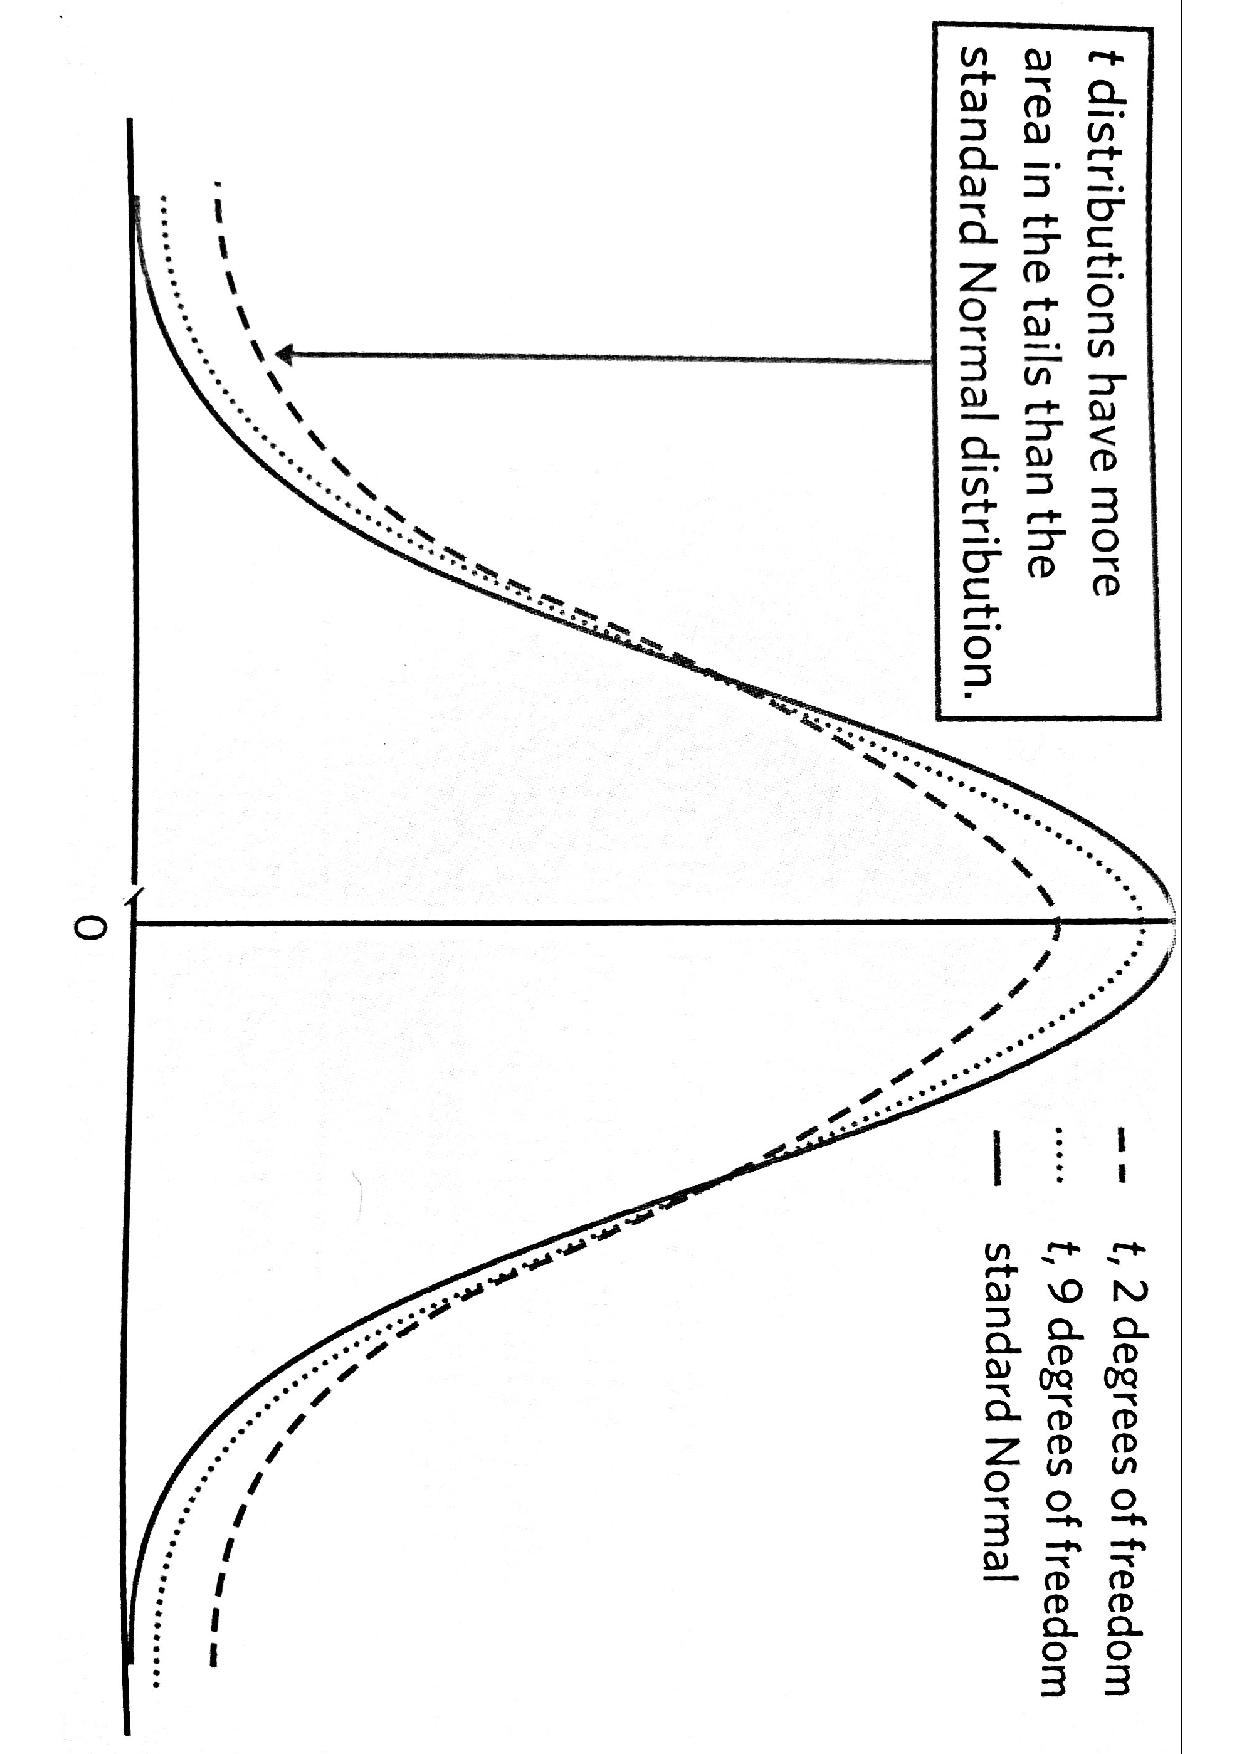
\includegraphics[scale=0.33, angle=90]{t_normal_comparison.pdf}
			\caption{Density curves for the $t$ distribution with 2 and 9 degrees of freedom and for the standard Normal distribution. All are symmetric with center 0. The $t$ distributions are somewhat more spread out.}
		\end{figure}
	}
	
\end{frame}


\begin{frame}[fragile]{$t_{(5)}$ distribution vs. Standard Normal distribution}
	\begin{minipage}{0.47\textwidth}
\begin{knitrout}\tiny
\definecolor{shadecolor}{rgb}{0.969, 0.969, 0.969}\color{fgcolor}\begin{kframe}
\begin{alltt}
\hlkwd{library}\hlstd{(mosaic)}
\hlkwd{xqnorm}\hlstd{(}\hlkwc{p} \hlstd{=} \hlkwd{c}\hlstd{(}\hlnum{0.025}\hlstd{,} \hlnum{0.975}\hlstd{))}
\end{alltt}
\end{kframe}
\end{knitrout}
\begin{knitrout}\tiny
\definecolor{shadecolor}{rgb}{0.969, 0.969, 0.969}\color{fgcolor}

{\centering 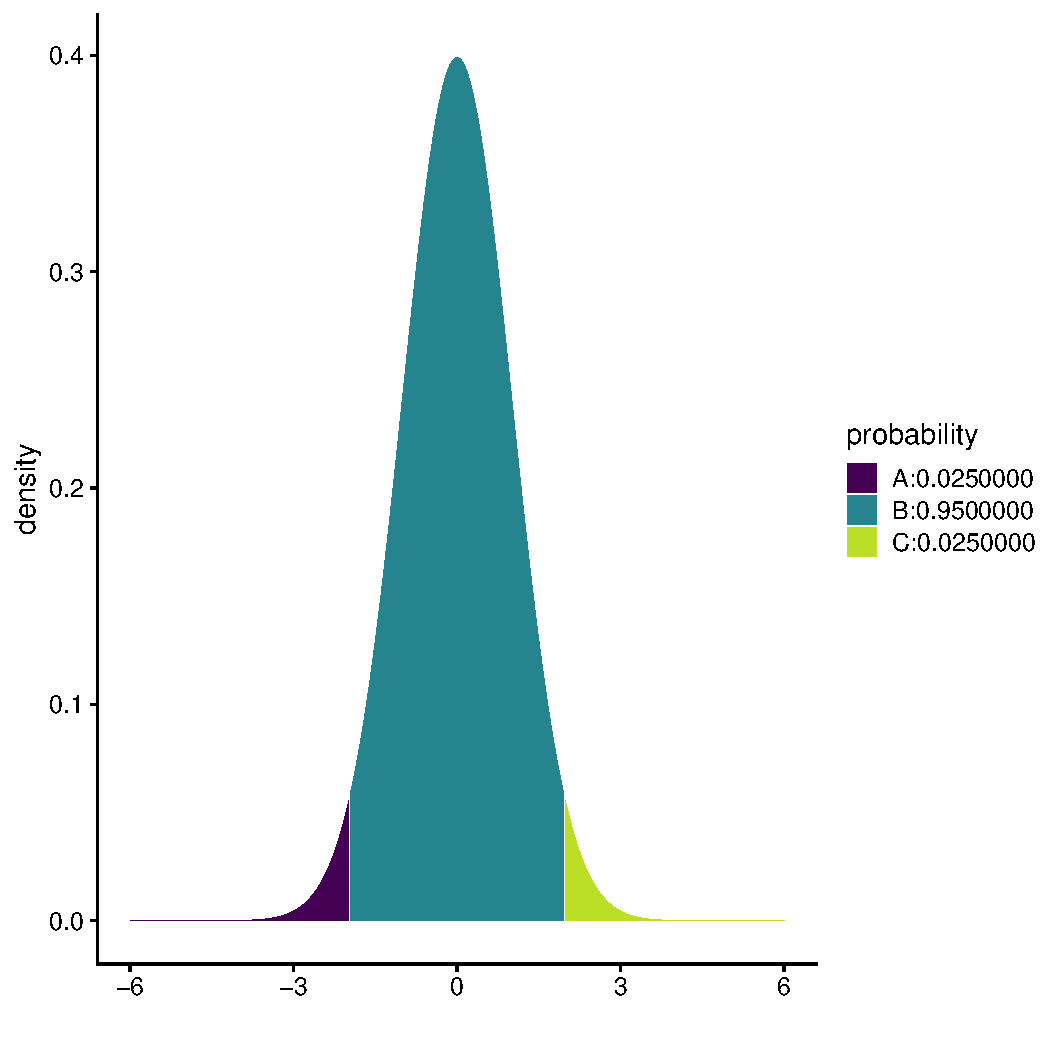
\includegraphics[width=\maxwidth]{figure/unnamed-chunk-3-1} 

}


\begin{kframe}\begin{verbatim}
## [1] -1.959964  1.959964
\end{verbatim}
\end{kframe}
\end{knitrout}
	\end{minipage}
	\begin{minipage}{0.5\textwidth}
\begin{knitrout}\tiny
\definecolor{shadecolor}{rgb}{0.969, 0.969, 0.969}\color{fgcolor}\begin{kframe}
\begin{alltt}
\hlkwd{library}\hlstd{(mosaic)}
\hlkwd{xqt}\hlstd{(}\hlkwc{p} \hlstd{=} \hlkwd{c}\hlstd{(}\hlnum{0.025}\hlstd{,} \hlnum{0.975}\hlstd{),} \hlkwc{df} \hlstd{=} \hlnum{5}\hlstd{)}
\end{alltt}
\end{kframe}

{\centering 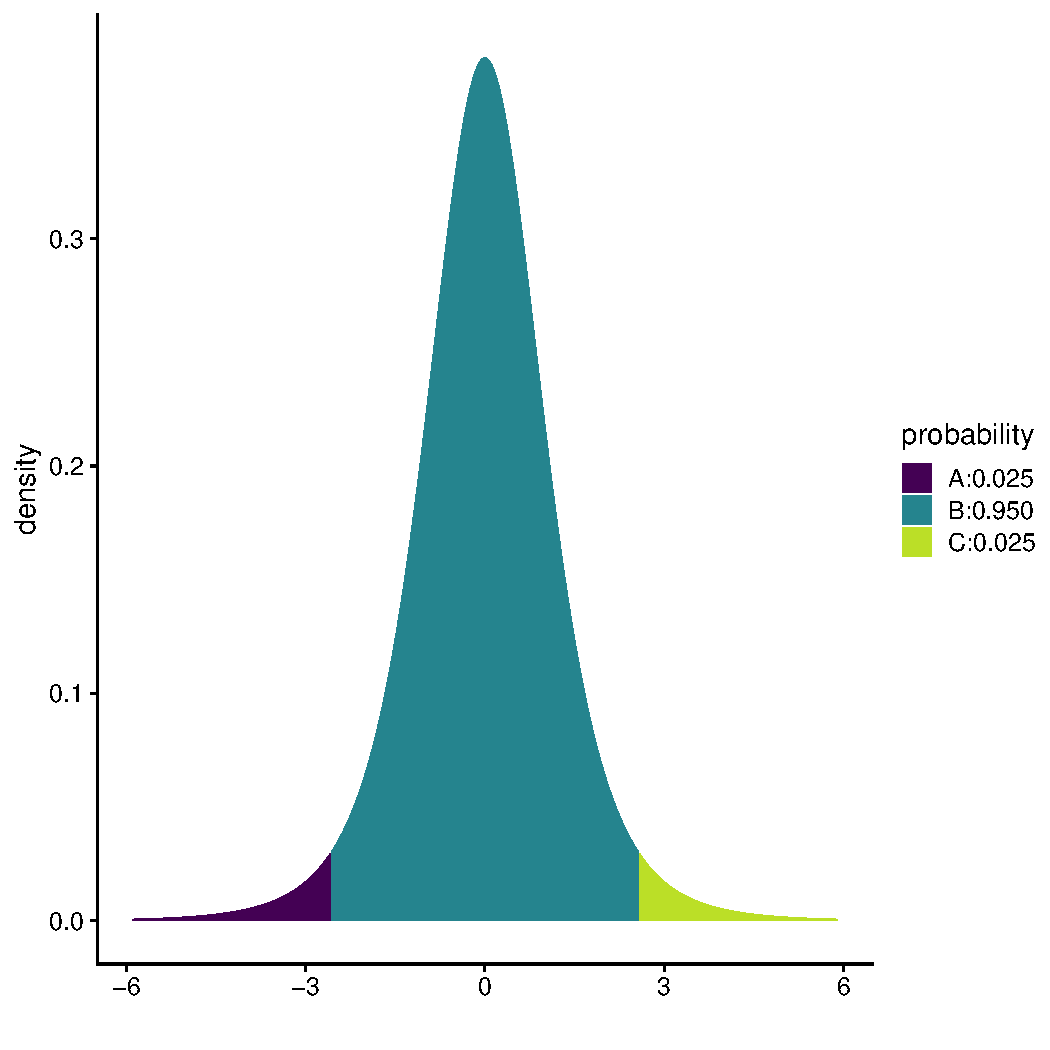
\includegraphics[width=\maxwidth]{figure/unnamed-chunk-4-1} 

}


\begin{kframe}\begin{verbatim}
## [1] -2.570582  2.570582
\end{verbatim}
\end{kframe}
\end{knitrout}
	\end{minipage}
\end{frame}



\begin{frame}[fragile]{$t_{(30)}$ distribution vs. Standard Normal distribution}
	\begin{minipage}{0.47\textwidth}
\begin{knitrout}\tiny
\definecolor{shadecolor}{rgb}{0.969, 0.969, 0.969}\color{fgcolor}\begin{kframe}
\begin{alltt}
\hlkwd{library}\hlstd{(mosaic)}
\hlkwd{xqnorm}\hlstd{(}\hlkwc{p} \hlstd{=} \hlkwd{c}\hlstd{(}\hlnum{0.025}\hlstd{,} \hlnum{0.975}\hlstd{))}
\end{alltt}
\end{kframe}
\end{knitrout}
\begin{knitrout}\tiny
\definecolor{shadecolor}{rgb}{0.969, 0.969, 0.969}\color{fgcolor}

{\centering 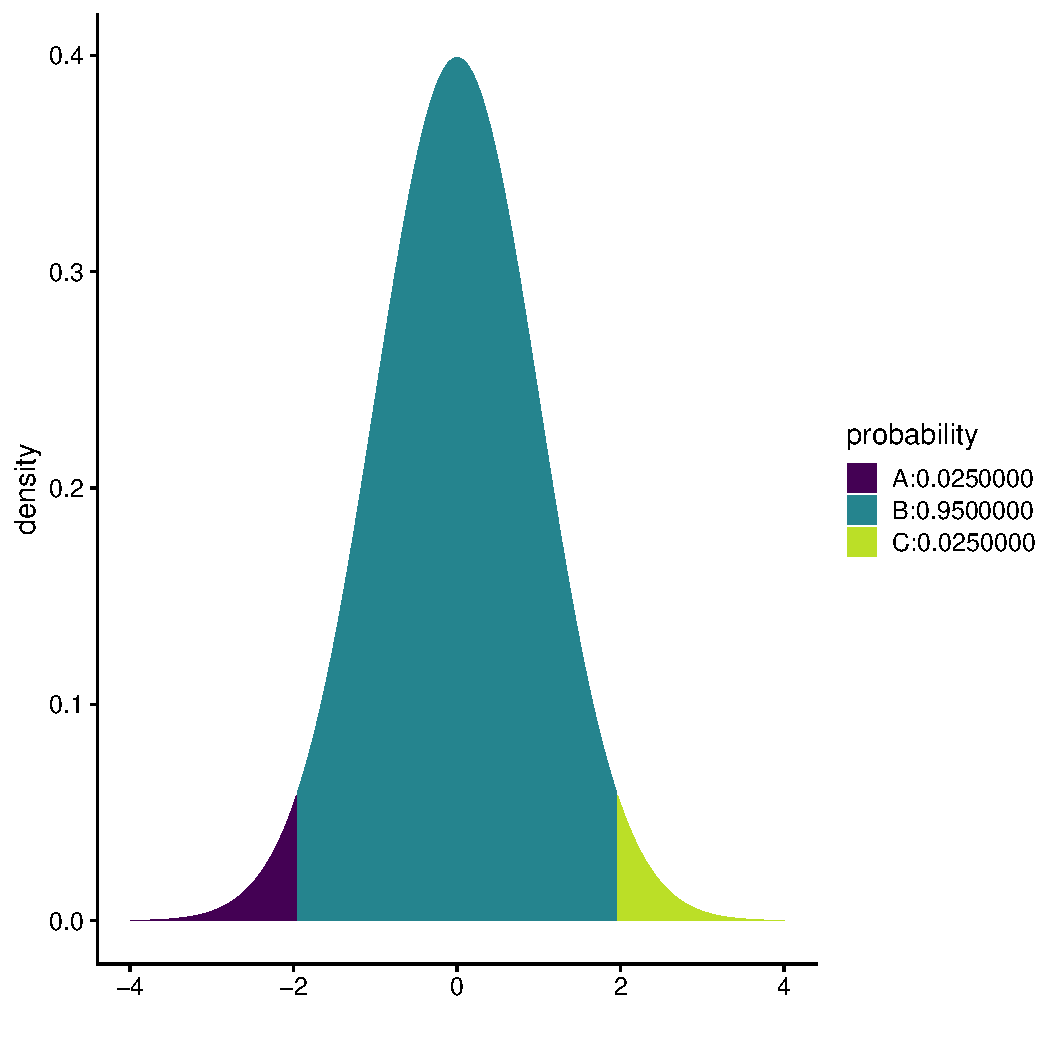
\includegraphics[width=\maxwidth]{figure/unnamed-chunk-6-1} 

}


\begin{kframe}\begin{verbatim}
## [1] -1.959964  1.959964
\end{verbatim}
\end{kframe}
\end{knitrout}
	\end{minipage}
	\begin{minipage}{0.5\textwidth}
\begin{knitrout}\tiny
\definecolor{shadecolor}{rgb}{0.969, 0.969, 0.969}\color{fgcolor}\begin{kframe}
\begin{alltt}
\hlkwd{library}\hlstd{(mosaic)}
\hlkwd{xqt}\hlstd{(}\hlkwc{p} \hlstd{=} \hlkwd{c}\hlstd{(}\hlnum{0.025}\hlstd{,} \hlnum{0.975}\hlstd{),} \hlkwc{df} \hlstd{=} \hlnum{30}\hlstd{)}
\end{alltt}
\end{kframe}
\end{knitrout}
\begin{knitrout}\tiny
\definecolor{shadecolor}{rgb}{0.969, 0.969, 0.969}\color{fgcolor}

{\centering 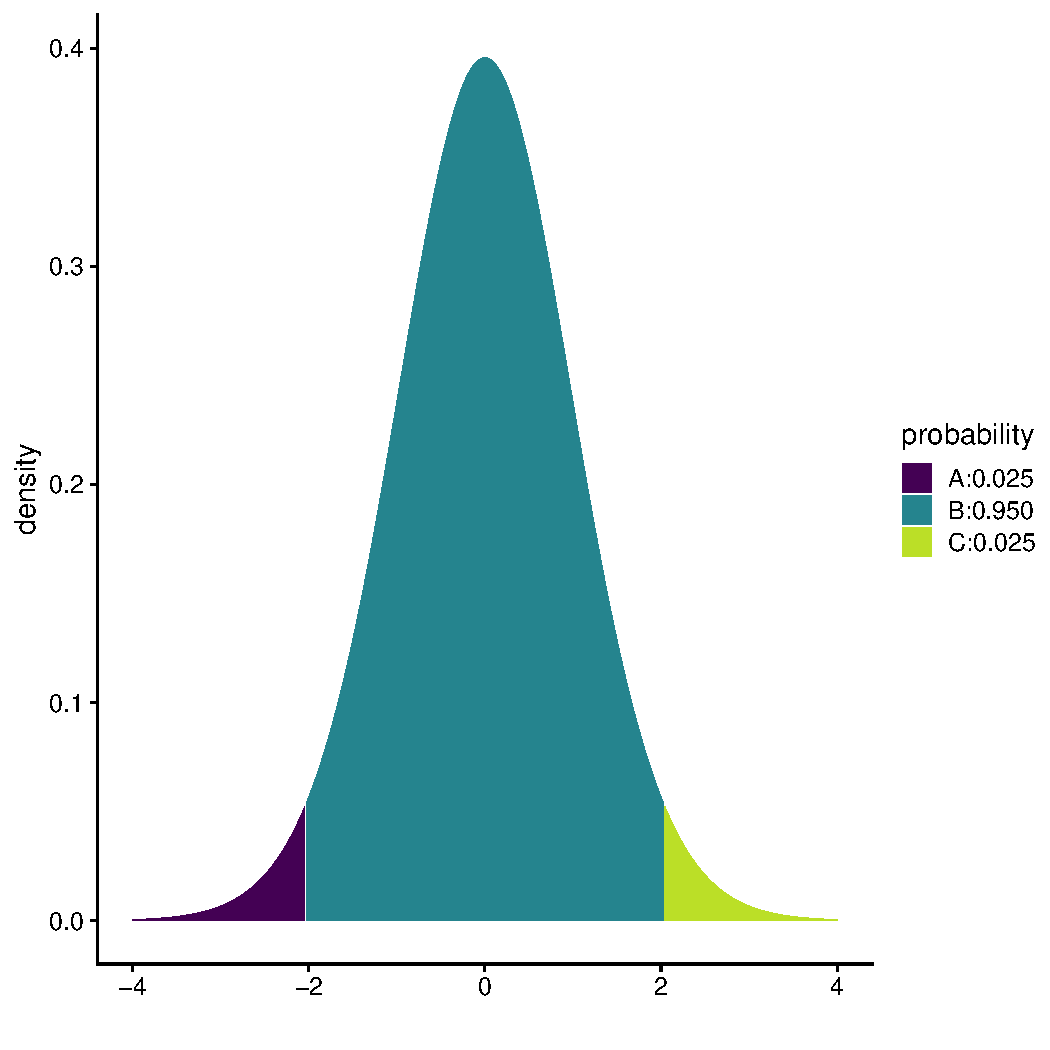
\includegraphics[width=\maxwidth]{figure/unnamed-chunk-8-1} 

}


\begin{kframe}\begin{verbatim}
## [1] -2.042272  2.042272
\end{verbatim}
\end{kframe}
\end{knitrout}
	\end{minipage}
\end{frame}

%\frame{\frametitle{$t$ distributions}
%	\begin{figure}
%		\begin{center}
%			\epsfig{figure=Tables/psls_table_C.eps,scale=.35}
%		\end{center}
%	\end{figure}
%}


\begin{frame}{$t$ distributions}
	\begin{itemize}
		\small
		\item Is symmetric around 0 ( just like the $\mathcal{N}(0,1)$ )
		\item Has a shape like that of the Z distribution, but with a SD slightly larger than
		unity i.e. slightly flatter and heavier-tailed
		\item Shape becomes indistinguishable from Z distribution as $n \rightarrow \infty$ (in fact as $n$ goes much beyond 30)
		\item Instead of  $\pm 1.96 \times  $ SEM for 95\% confidence (or to use as the critical value in a null-hypothesis test), we need these multiples (or critical values): \\ \ \\
		
		\begin{tabular}{r r r r}
			$n$ & `degrees of freedom' & Multiple & from \texttt{R} \\ 
			\hline
			2 & 1 & 12.71 & \texttt{qt(0.975,  1)} \\
			3 & 2 & 4.30 & \texttt{qt(0.975,  2)}\\
			4 & 3 & 3.18 & \texttt{qt(0.975,  3)}\\
			11 &10 & 2.23 & \texttt{qt(0.975, 10)}  \\
			21 & 20 & 2.09 & \texttt{qt(0.975, 20)} \\
			31 & 30 & 2.04 & \texttt{qt(0.975, 30)} \\
			121 & 120 & 1.98 & \texttt{qt(0.975,120)} \\
			$\infty$ & $\infty$ & 1.96 & \texttt{qt(0.975,Inf)}   \\
		\end{tabular}
		
	\end{itemize}
\end{frame}



\begin{frame}[fragile]{$t$ distributions}
	Sample size increases $\rightarrow$ degrees of freedom increase $\rightarrow$ $t$ starts to look like $\mathcal{N}(0,1)$
\begin{knitrout}\tiny
\definecolor{shadecolor}{rgb}{0.969, 0.969, 0.969}\color{fgcolor}

{\centering 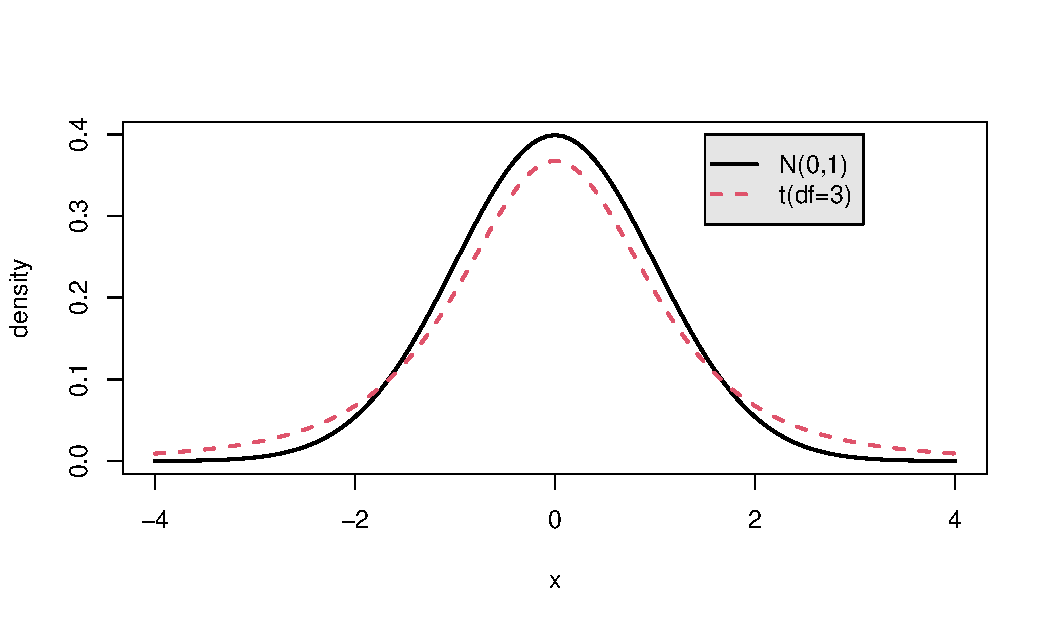
\includegraphics[width=\maxwidth]{figure/unnamed-chunk-9-1} 

}


\end{knitrout}
\end{frame}

\begin{frame}[fragile]{$t$ distributions}
	Sample size increases $\rightarrow$ degrees of freedom increase $\rightarrow$ $t$ starts to look like $\mathcal{N}(0,1)$
\begin{knitrout}\tiny
\definecolor{shadecolor}{rgb}{0.969, 0.969, 0.969}\color{fgcolor}

{\centering 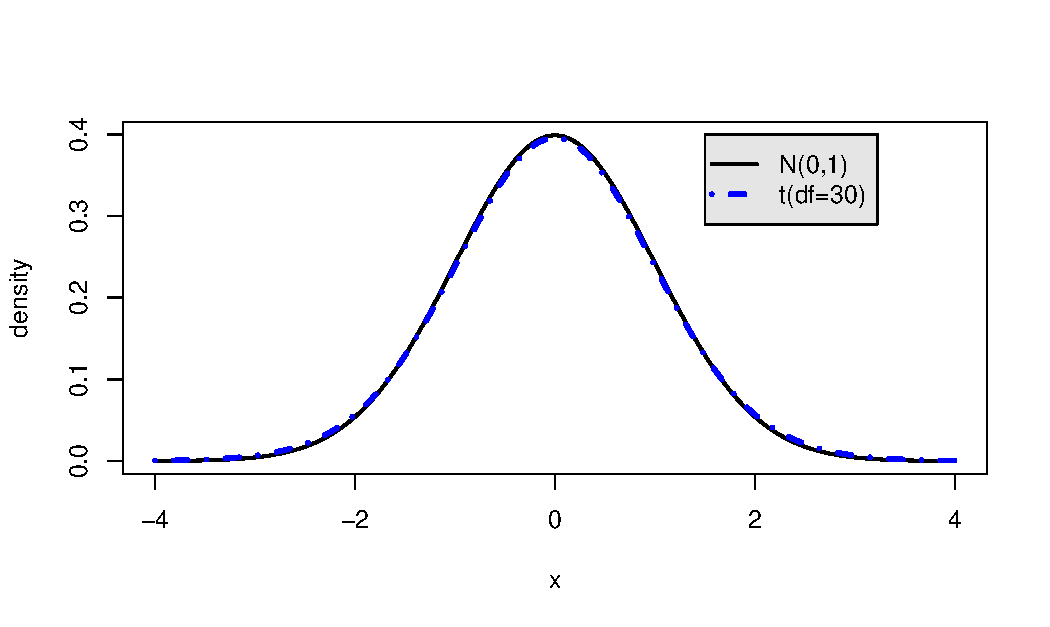
\includegraphics[width=\maxwidth]{figure/unnamed-chunk-10-1} 

}


\end{knitrout}
	
	\Large This is where the infamous $n=30$ comes from !!
\end{frame}

\frame{\frametitle{$t$ procedures} We can calculate CIs and
	perform significance tests much as before (example coming up
	soon).\\\ \\
	
	A significance test of a single sample mean using the $t$-statistic
	is called a \textcolor{blue}{one-sample $t$-test}. \\ \ \\
	
	Collectively, the significance tests and confidence-interval based
	tests using the $t$ distribution are called \underline{$t$ procedures}.  \\ \ \\
	
}

\begin{frame}{The one-sample $t$ test}
	
	\Wider[4em]{
		\centering
		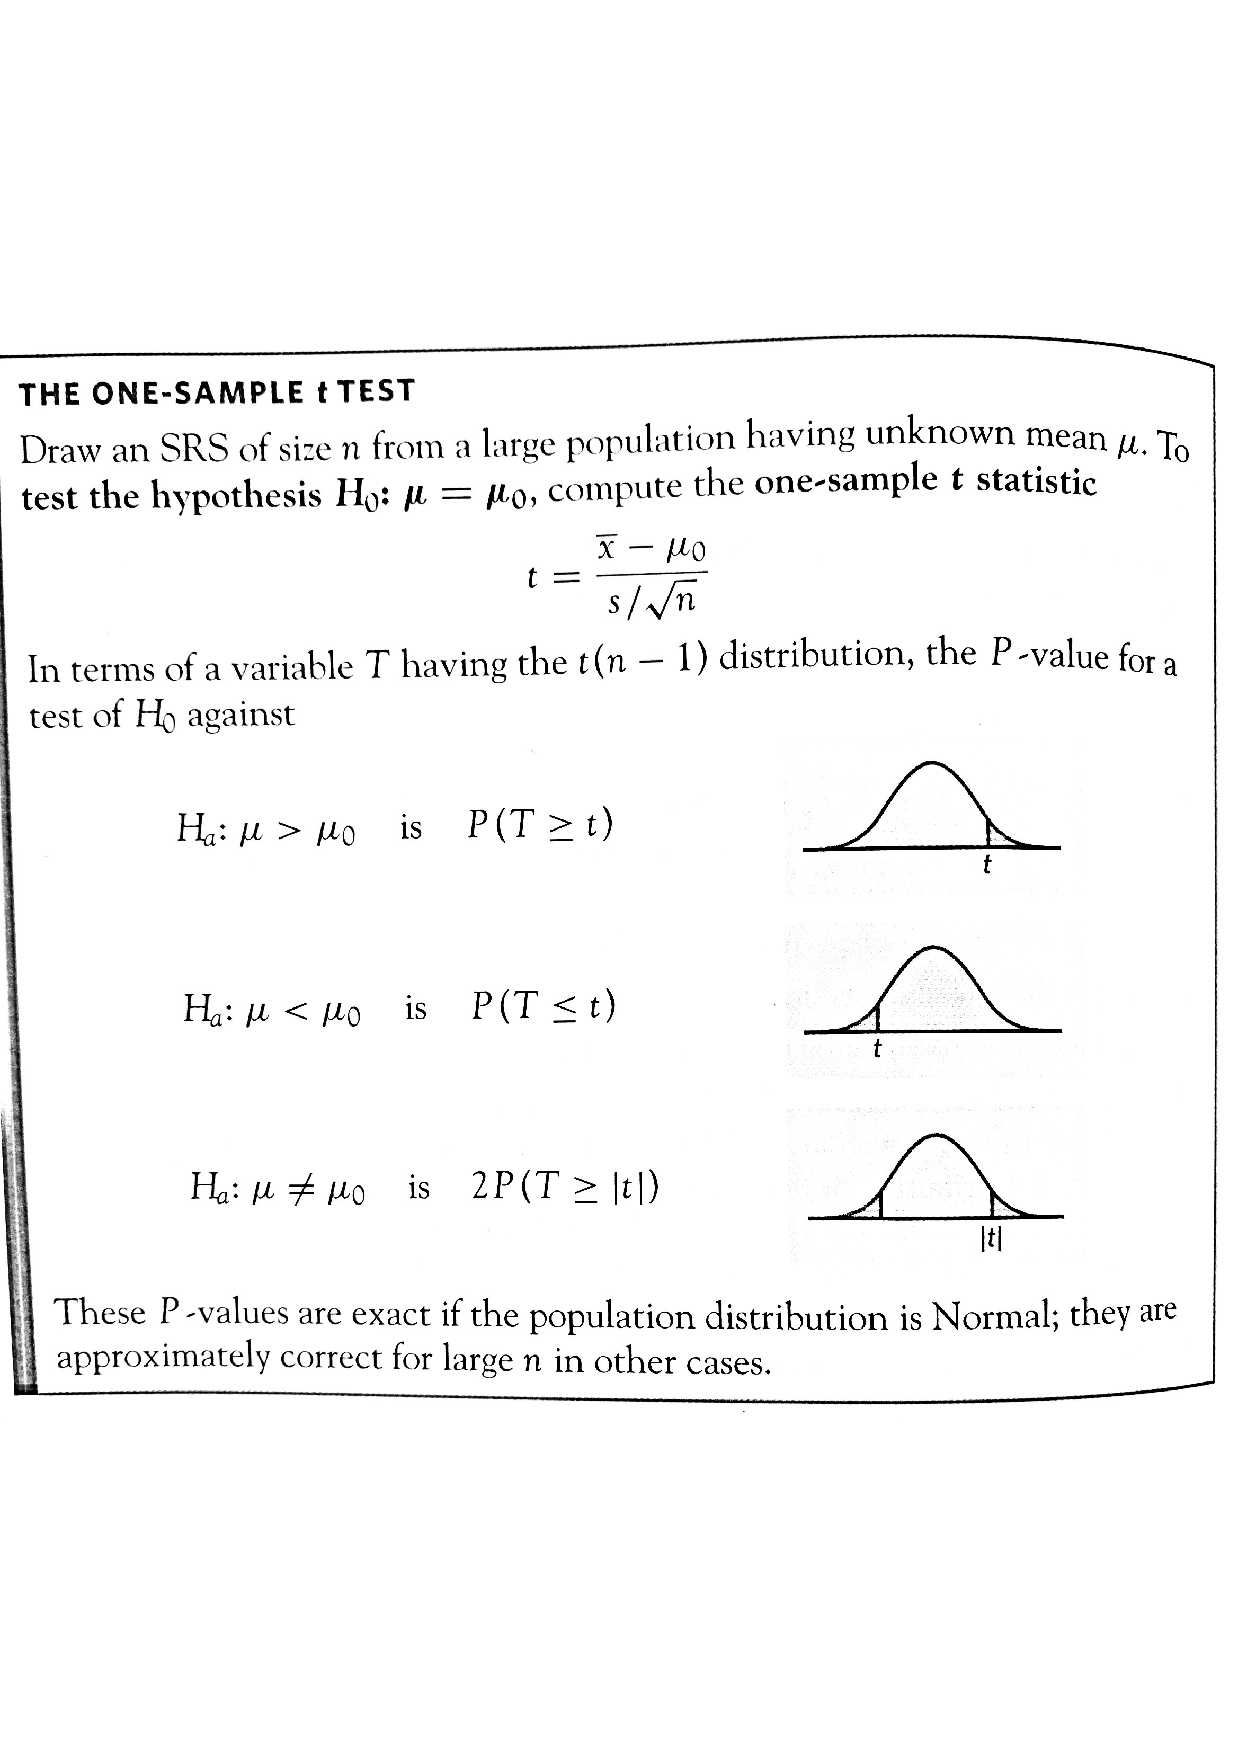
\includegraphics[scale=0.35]{ttest.pdf}
		
	}
	
\end{frame}


\begin{frame}{A note about the conditions for $t$ procedures}
	
	\begin{itemize}
		\setlength\itemsep{1em}
		\item B\&M stress that the \textbf{first} of their conditions as \textit{very important}: \textit{we can regard} our data as a simple random sample (SRS) from  the population \pause 
		\item The \textbf{second}, observations from the population have a \textit{\underline{Normal}} distribution with unknown mean parameter $\mu$ and unknown standard deviation parameter $\sigma$ less so 
		\item \textit{In practice}, inference procedures \textit{can accommodate some deviations from
			the Normality condition} when the sample is large enough. 
	\end{itemize}
\end{frame}


\frame{\frametitle{Robustness of the $t$ procedures} A statistical
	procedure is said to be \textbf{robust} if it is insensitive to
	violations of the assumptions made. \\ \ \\
	\begin{itemize}
		\setlength\itemsep{1em}
		%\item Results of $t$ procedures (CIs, significance tests) are exact if the
		%population from which the simple random sample was drawn is Normal. \pause
		\item $t$ procedures are not robust against \textit{extreme}
		skewness, \underline{in small samples}, since the procedures are
		based on using $\overline{y}$ and $s$ (which are sensitive to
		outliers).
		\item Recall: \textcolor{blue}{Unless there is a very compelling reason
			(e.g.~known/confirmed error in the recorded data), outliers should not be discarded.}
		
	\end{itemize}
} \frame{\frametitle{Robustness of the $t$ procedures}
	\begin{itemize}
		\setlength\itemsep{2em}
		\item $t$ procedures \textbf{are} robust against other forms
		of non-normality and, even with considerable skew, perform well when $n$ is large. Why?
		\pause
		\item When $n$ is large, $s$ is a good estimate of $\sigma$
		(recall that $s$ is unbiased and, like most estimates, precision
		improves with increasing sample size) \pause
		\item CLT: $\overline{y}$ will be Normal when $n$ is large, even if the
		population data are not
		
		
	\end{itemize}
}



\begin{frame}{When and why we use the $t$-distribution}
	\mylist{When $\sigma$ is unknown use $t$ distribution. \blue{but why?}; \pause the spread of the $t$ distribution is greater than $\mathcal{N}(0,1)$  }
\end{frame}



\begin{frame}[fragile]{Rejecting the Null ($H_0: \mu = \mu_0$) when $\sigma$ is known}
	\small
	\[ \underbrace{z_{0.975}}_{\textrm{critical value}}=1.96 = \frac{\bar{y}-\mu_0}{\sigma/\sqrt{n}} \rightarrow \frac{1.96 }{\sqrt{n}}\sigma = \bar{y}-\mu_0   \] which means that to reject $H_0$ the difference between your sample mean and $\mu_0$ needs to be \blue{greater than $\frac{1.96}{\sqrt{n}}$ standard deviations} 

\begin{knitrout}\tiny
\definecolor{shadecolor}{rgb}{0.969, 0.969, 0.969}\color{fgcolor}\begin{kframe}
\begin{alltt}
\hlstd{mosaic}\hlopt{::}\hlkwd{xqnorm}\hlstd{(}\hlkwc{p} \hlstd{=} \hlkwd{c}\hlstd{(}\hlnum{0.025}\hlstd{,} \hlnum{0.975}\hlstd{))}
\end{alltt}
\end{kframe}

{\centering 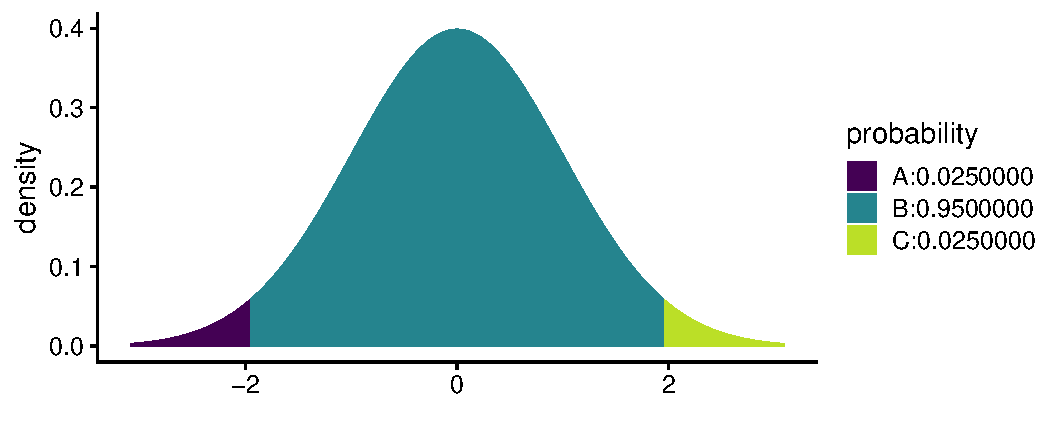
\includegraphics[width=\maxwidth]{figure/unnamed-chunk-12-1} 

}


\begin{kframe}\begin{verbatim}
## [1] -1.959964  1.959964
\end{verbatim}
\end{kframe}
\end{knitrout}
\end{frame}



\begin{frame}[fragile]{Rejecting the Null ($H_0: \mu = \mu_0$) when $\sigma$ is unknown}
	\small
	\[ \underbrace{t_{0.975,df=3}^\star}_{\textrm{critical value}}=3.18 = \frac{\bar{y}-\mu_0}{s/\sqrt{n}} \rightarrow  \frac{3.18}{\sqrt{n}}s = \bar{y}-\mu_0   \] which means that to reject $H_0$ the difference between your sample mean and $\mu_0$ needs to be \blue{greater than $\frac{3.18}{\sqrt{n}}$ standard deviations} 

	
\begin{knitrout}\tiny
\definecolor{shadecolor}{rgb}{0.969, 0.969, 0.969}\color{fgcolor}\begin{kframe}
\begin{alltt}
\hlstd{mosaic}\hlopt{::}\hlkwd{xqt}\hlstd{(}\hlkwc{p} \hlstd{=} \hlkwd{c}\hlstd{(}\hlnum{0.025}\hlstd{,} \hlnum{0.975}\hlstd{),} \hlkwc{df} \hlstd{=} \hlnum{3}\hlstd{)}
\end{alltt}
\end{kframe}

{\centering 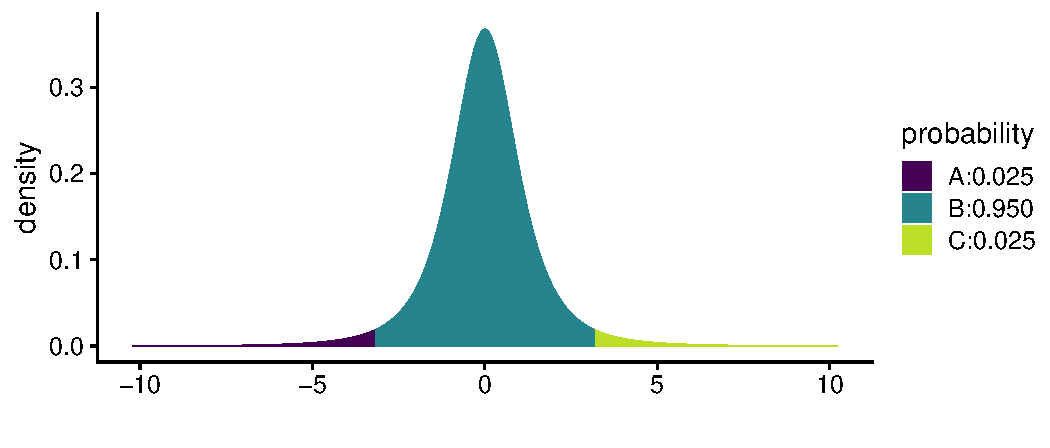
\includegraphics[width=\maxwidth]{figure/unnamed-chunk-14-1} 

}


\begin{kframe}\begin{verbatim}
## [1] -3.182446  3.182446
\end{verbatim}
\end{kframe}
\end{knitrout}
	
\end{frame}




\begin{frame}{Summary of $t$ distribution}
	\mylist{Its harder to reject the null when using the $t$ distribution; \pause Confidence intervals are also wider; \pause This is due to our uncertainty about the estimated variance ;\pause Larger samples lead to more accurate estimates of $\sigma$; \pause This is reflected in the fact that there is a different $t$ distribution for each sample size  ; \pause As $n \rightarrow \infty$, sample standard deviation $s$ gets closer to $\sigma$; \pause As degrees of freedom increase, $t$ distribution gets closer to Normal distribution}
\end{frame}


\section{Examples}


\begin{frame}{Application: How fast is your reaction time?}
	\small\url{https://faculty.washington.edu/chudler/java/redgreen.html} 
	
	\framedgraphic{JHReactionTimes.png}
	
\end{frame}


\begin{frame}[fragile]{Application: How fast is your reaction time?}
\begin{knitrout}\tiny
\definecolor{shadecolor}{rgb}{0.969, 0.969, 0.969}\color{fgcolor}\begin{kframe}
\begin{alltt}
\hlstd{reaction.times} \hlkwb{<-} \hlkwd{c}\hlstd{(}\hlnum{325}\hlstd{,}\hlnum{327}\hlstd{,}\hlnum{357}\hlstd{,}\hlnum{299}\hlstd{,}\hlnum{378}\hlstd{)}\hlopt{/}\hlnum{1000}
\hlkwd{summary}\hlstd{(reaction.times)}
\end{alltt}
\begin{verbatim}
##    Min. 1st Qu.  Median    Mean 3rd Qu.    Max. 
##  0.2990  0.3250  0.3270  0.3372  0.3570  0.3780
\end{verbatim}
\begin{alltt}
\hlkwd{round}\hlstd{(}\hlkwd{sd}\hlstd{(reaction.times),}\hlnum{3}\hlstd{)}
\end{alltt}
\begin{verbatim}
## [1] 0.031
\end{verbatim}
\begin{alltt}
\hlkwd{length}\hlstd{(reaction.times)}
\end{alltt}
\begin{verbatim}
## [1] 5
\end{verbatim}
\end{kframe}
\end{knitrout}
	
\end{frame}


\begin{frame}[fragile]{5 ways of calculating a confidence interval}
	
	We are interested in calculating a 95\% confidence interval for the mean reaction time based on the sample of 5 reaction times. \\ \ \\
	\pause
	Five ways of doing this:
	\begin{enumerate}
		\setlength\itemsep{1em}
		\item By hand (using the $\pm$ formula and \texttt{R} as a calculator)
		\item Using the quantile function for the $t$ distribution \texttt{stats::qt}
		\item Fitting an intercept-only regression model ($y = \beta_0 + \varepsilon$)
		\item Using a canned function (\texttt{mosaic::t.test}, \texttt{stats::t.test})
		\item Bootstrap
	\end{enumerate}
	
\end{frame}

\begin{frame}[fragile]{1. By hand using the $\pm$ formula}
\begin{knitrout}\tiny
\definecolor{shadecolor}{rgb}{0.969, 0.969, 0.969}\color{fgcolor}\begin{kframe}
\begin{alltt}
\hlstd{n} \hlkwb{<-} \hlkwd{length}\hlstd{(reaction.times)}
\hlstd{SEM} \hlkwb{<-} \hlkwd{sd}\hlstd{(reaction.times)}\hlopt{/}\hlkwd{sqrt}\hlstd{(n)}
\end{alltt}
\begin{verbatim}
## [1] 0.01372734
\end{verbatim}
\begin{alltt}
\hlstd{ybar} \hlkwb{<-} \hlkwd{mean}\hlstd{(reaction.times)}
\end{alltt}
\begin{verbatim}
## [1] 0.3372
\end{verbatim}
\begin{alltt}
\hlstd{multiple.for.95pct} \hlkwb{<-} \hlstd{stats}\hlopt{::}\hlkwd{qt}\hlstd{(}\hlkwc{p} \hlstd{=} \hlkwd{c}\hlstd{(}\hlnum{0.025}\hlstd{,} \hlnum{0.975}\hlstd{),} \hlkwc{df} \hlstd{= n}\hlopt{-}\hlnum{1}\hlstd{)}
\end{alltt}
\begin{verbatim}
## [1] -2.776445  2.776445
\end{verbatim}
\begin{alltt}
\hlstd{by_hand_CI} \hlkwb{<-} \hlstd{ybar} \hlopt{+} \hlstd{multiple.for.95pct} \hlopt{*} \hlstd{SEM}
\end{alltt}
\begin{verbatim}
## [1] 0.29909 0.37531
\end{verbatim}
\end{kframe}
\end{knitrout}
\end{frame}

\begin{frame}[fragile]{2. Using \texttt{stats::qt}}
	\textit{Note: \texttt{R} only provides the standard $t$ distribution. In order to get a scaled version we must define our own function.}
	
	\vspace*{0.2in}
	
\begin{knitrout}\tiny
\definecolor{shadecolor}{rgb}{0.969, 0.969, 0.969}\color{fgcolor}\begin{kframe}
\begin{alltt}
\hlstd{n} \hlkwb{<-} \hlkwd{length}\hlstd{(reaction.times)}
\hlstd{SEM} \hlkwb{<-} \hlkwd{sd}\hlstd{(reaction.times)}\hlopt{/}\hlkwd{sqrt}\hlstd{(n)}
\hlstd{ybar} \hlkwb{<-} \hlkwd{mean}\hlstd{(reaction.times)}

\hlcom{# scaled version of the standard t distribution}
\hlstd{qt_ls} \hlkwb{<-} \hlkwa{function}\hlstd{(}\hlkwc{p}\hlstd{,} \hlkwc{df}\hlstd{,} \hlkwc{mean}\hlstd{,} \hlkwc{sd}\hlstd{)} \hlkwd{qt}\hlstd{(}\hlkwc{p} \hlstd{= p,} \hlkwc{df} \hlstd{= df)} \hlopt{*} \hlstd{sd} \hlopt{+} \hlstd{mean}

\hlkwd{qt_ls}\hlstd{(}\hlkwc{p} \hlstd{=} \hlkwd{c}\hlstd{(}\hlnum{0.025}\hlstd{,} \hlnum{0.975}\hlstd{),} \hlkwc{df} \hlstd{= n} \hlopt{-} \hlnum{1}\hlstd{,} \hlkwc{mean} \hlstd{= ybar,} \hlkwc{sd} \hlstd{= SEM)}
\end{alltt}
\begin{verbatim}
## [1] 0.2990868 0.3753132
\end{verbatim}
\end{kframe}
\end{knitrout}
\end{frame}


\begin{frame}[fragile]{3. Fitting an intercept-only regression model}
\begin{knitrout}\tiny
\definecolor{shadecolor}{rgb}{0.969, 0.969, 0.969}\color{fgcolor}\begin{kframe}
\begin{alltt}
\hlstd{fit} \hlkwb{<-} \hlstd{stats}\hlopt{::}\hlkwd{lm}\hlstd{(reaction.times} \hlopt{~} \hlnum{1}\hlstd{)}
\hlkwd{summary}\hlstd{(fit)}
\end{alltt}
\begin{verbatim}
## Coefficients:
##             Estimate Std. Error t value Pr(>|t|)    
## (Intercept)  0.33720    0.01373   24.56 1.63e-05 ***
## ---
## Signif. codes:  0 '***' 0.001 '**' 0.01 '*' 0.05 '.' 0.1 ' ' 1
## 
## Residual standard error: 0.0307 on 4 degrees of freedom
\end{verbatim}
\begin{alltt}
\hlstd{stats}\hlopt{::}\hlkwd{confint}\hlstd{(fit)}
\end{alltt}
\begin{verbatim}
##                 2.5 %    97.5 %
## (Intercept) 0.2990868 0.3753132
\end{verbatim}
\end{kframe}
\end{knitrout}
\end{frame}


\begin{frame}[fragile]{3. Fitting an intercept-only regression model}
	In the regression output:
	\begin{itemize}
		\setlength\itemsep{1em}
		\item \texttt{Estimate}: the mean reaction time (an estimate of the intercept $\beta_0$)
		\item \texttt{t value}: the test statistic 
		\item \texttt{Std. Error}: the standard error of the mean (SEM)
		\item \texttt{Pr(>|t|)}: is the $p$-value
	\end{itemize} 
	
	
\end{frame}


\begin{frame}[fragile]{3. Fitting an intercept-only regression model}
	

	
	\small
	These are based on the (useless) null hypothesis $H_0: \mu_0 = 0$ \\ \ \\
	
	\begin{itemize}
		\item \texttt{t value} = $\frac{\bar{y} - \mu_0}{s / \sqrt{n}}$ = $\frac{0.33720 - 0}{0.01373}$ = 24.56
		\item \texttt{Pr(>|t|)} \\ \ \\
		= $P(\textrm{t value} > t_{(n-1)}) + P(-\textrm{t value} < t_{(n-1)})$ \\ \ \\
		= \small{\texttt{pt(q = 24.56, df = n-1, lower.tail = FALSE)} +  \texttt{pt(q = -24.56, df = n-1)}} \\ \ \\
		= \ensuremath{8.155\times 10^{-6}} + \ensuremath{8.155\times 10^{-6}} = \ensuremath{1.631\times 10^{-5}}
	\end{itemize}
	
	
\end{frame}



\begin{frame}[fragile]{4. Canned function}
	
\begin{knitrout}\tiny
\definecolor{shadecolor}{rgb}{0.969, 0.969, 0.969}\color{fgcolor}\begin{kframe}
\begin{alltt}
\hlstd{stats}\hlopt{::}\hlkwd{t.test}\hlstd{(reaction.times)}
\end{alltt}
\begin{verbatim}
## One Sample t-test with reaction.times 
## t = 24.6, df = 4, p-value = 1.63e-05
## alternative hypothesis: true mean is not equal to 0 
## 95 percent confidence interval:
##  0.299 0.375 
## sample estimates:
## mean of x 
##     0.337
\end{verbatim}
\end{kframe}
\end{knitrout}
	
\end{frame}



\begin{frame}[fragile]{5. Bootstrap}
	
\begin{knitrout}\tiny
\definecolor{shadecolor}{rgb}{0.969, 0.969, 0.969}\color{fgcolor}\begin{kframe}
\begin{alltt}
\hlstd{df_react} \hlkwb{<-} \hlkwd{data.frame}\hlstd{(reaction.times)} \hlcom{# need data.frame to bootstrap}
\hlstd{B} \hlkwb{<-} \hlnum{10000} \hlstd{; N} \hlkwb{<-} \hlkwd{nrow}\hlstd{(df_react)}
\hlstd{R} \hlkwb{<-} \hlkwd{replicate}\hlstd{(B, \{}
  \hlstd{dplyr}\hlopt{::}\hlkwd{sample_n}\hlstd{(df_react,} \hlkwc{size} \hlstd{= N,} \hlkwc{replace} \hlstd{=} \hlnum{TRUE}\hlstd{)} \hlopt
  \hlstd{dplyr}\hlopt{::}\hlkwd{summarize}\hlstd{(}\hlkwc{r} \hlstd{=} \hlkwd{mean}\hlstd{(reaction.times))} \hlopt
  \hlstd{dplyr}\hlopt{::}\hlkwd{pull}\hlstd{(r)}
\hlstd{\})}
\end{alltt}
\begin{verbatim}
##  2.5% 97.5% 
## 0.315 0.363
\end{verbatim}
\end{kframe}

{\centering 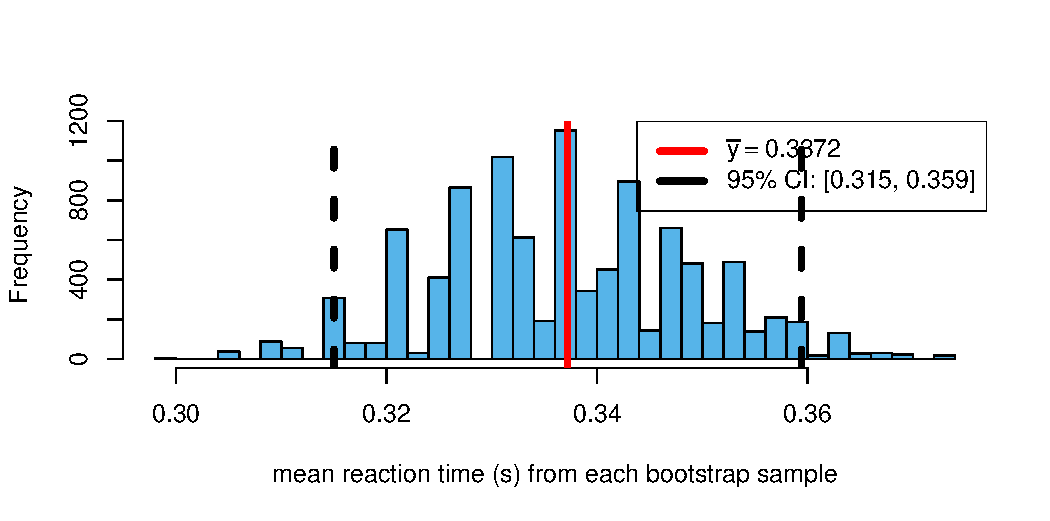
\includegraphics[width=\maxwidth]{figure/unnamed-chunk-21-1} 

}


\end{knitrout}
	
\end{frame}


\begin{frame}{Summary}
	\begin{itemize}
		\setlength\itemsep{1em}
		\item We use $t$ procedures instead of $Z$ when we have very small samples ($n \leq 30$)
		\item This is because our estimate of $\sigma$ is probably not accurate with such a small sample
		\item We account for this extra uncertainty by widening the interval $\to$ larger multiplicative factor ($t_{(n-1)}$ > $z^\star$) \pause 
		\item Reality check: It is unlikely you will have such a small sample unless you're working with rats
		\item In practice you don't need to worry about $t$ vs. $Z$. The software does it for you.
		\item However, you should still understand where the numbers are coming from and how it is being calculated. Computers aren't intelligent, they're just well trained. 
	\end{itemize}
\end{frame}


\begin{frame}[fragile]{Session Info}
	\tiny
	
\begin{knitrout}\tiny
\definecolor{shadecolor}{rgb}{0.969, 0.969, 0.969}\color{fgcolor}\begin{kframe}
\begin{verbatim}
R version 4.0.4 (2021-02-15)
Platform: x86_64-pc-linux-gnu (64-bit)
Running under: Pop!_OS 21.04

Matrix products: default
BLAS:   /usr/lib/x86_64-linux-gnu/openblas-pthread/libblas.so.3
LAPACK: /usr/lib/x86_64-linux-gnu/openblas-pthread/libopenblasp-r0.3.13.so

attached base packages:
[1] tools     stats     graphics  grDevices utils     datasets  methods  
[8] base     

other attached packages:
 [1] latex2exp_0.4.0   DT_0.16           mosaic_1.7.0      Matrix_1.3-2     
 [5] mosaicData_0.20.1 ggformula_0.9.4   ggstance_0.3.4    lattice_0.20-41  
 [9] kableExtra_1.2.1  socviz_1.2        gapminder_0.3.0   here_0.1         
[13] NCStats_0.4.7     FSA_0.8.30        forcats_0.5.1     stringr_1.4.0    
[17] dplyr_1.0.7       purrr_0.3.4       readr_1.4.0       tidyr_1.1.3      
[21] tibble_3.1.3      ggplot2_3.3.5     tidyverse_1.3.0   knitr_1.33       

loaded via a namespace (and not attached):
 [1] fs_1.5.0           lubridate_1.7.9    webshot_0.5.2      httr_1.4.2        
 [5] rprojroot_2.0.2    backports_1.2.1    utf8_1.2.2         R6_2.5.1          
 [9] DBI_1.1.1          colorspace_2.0-2   withr_2.4.2        tidyselect_1.1.1  
[13] gridExtra_2.3      leaflet_2.0.3      curl_4.3.2         compiler_4.0.4    
[17] cli_3.0.1          rvest_1.0.0        pacman_0.5.1       xml2_1.3.2        
[21] ggdendro_0.1.22    labeling_0.4.2     mosaicCore_0.8.0   scales_1.1.1      
[25] digest_0.6.27      foreign_0.8-81     rmarkdown_2.9.7    rio_0.5.16        
[29] pkgconfig_2.0.3    htmltools_0.5.2    highr_0.9          dbplyr_1.4.4      
[33] fastmap_1.1.0      htmlwidgets_1.5.3  rlang_0.4.11       readxl_1.3.1      
[37] rstudioapi_0.13    farver_2.1.0       generics_0.1.0     jsonlite_1.7.2    
[41] crosstalk_1.1.1    zip_2.2.0          car_3.0-9          magrittr_2.0.1    
[45] Rcpp_1.0.7         munsell_0.5.0      fansi_0.5.0        abind_1.4-5       
[49] lifecycle_1.0.0    stringi_1.7.3      carData_3.0-4      MASS_7.3-53.1     
[53] plyr_1.8.6         grid_4.0.4         blob_1.2.1         ggrepel_0.8.2     
[57] crayon_1.4.1       cowplot_1.1.0      haven_2.3.1        splines_4.0.4     
[61] hms_1.0.0          pillar_1.6.2       reprex_0.3.0       glue_1.4.2        
[65] evaluate_0.14      data.table_1.14.0  modelr_0.1.8       vctrs_0.3.8       
[69] tweenr_1.0.1       cellranger_1.1.0   gtable_0.3.0       polyclip_1.10-0   
[73] assertthat_0.2.1   TeachingDemos_2.12 xfun_0.25          ggforce_0.3.2     
[77] openxlsx_4.1.5     broom_0.7.2        viridisLite_0.4.0  ellipsis_0.3.2    
\end{verbatim}
\end{kframe}
\end{knitrout}
	
\end{frame}

\end{document}
